\documentclass[12pt]{article}
\usepackage{graphicx}
\DeclareGraphicsExtensions{.pdf,.png,.jpg}

\title{A Scalable Data Integration and Entity Resolution Framework for Hadoop}

\author{Eric Peyton\\
\small Georgia Institute of Technology\\
\small CS 4365 Project Proposal\\
}

\begin{document}
\maketitle

\begin{abstract}
Data integration is the process of combining multiple data sources through an ETL procedure into a common unified view of the data. Integrating large datasets introduces a number of new challenges, especially if much of the data is noisy. These heterogenous data sources are manipulated to fit the common schema and loaded. Entity resolution is the process of resolving duplicated entities and relationships between them. This process may involve complex matching algorithms and machine learning.

I am proposing a Java framework to extend the Apache Hadoop library and facilitate smooth parallel data integration and entity resolution on a cluster. Hadoop provides a powerful platform for parallel computing. However, often many adjustments to an application are required in order to fit the MapReduce programming model. This typically involves much code and testing. For integrating data, this includes writing a custom MapReduce job for every new data source. To resolve entity duplicates, more MapReduce jobs have to written to match, unify, and merge the duplicate entities. The proposed Java framework will greatly simpifly this process and provide robust tools for integrating large data sources and deduplicating the results.
\end{abstract}
\section{Goals}
The goals of the project include:
\begin{itemize}
    \item Conciseness\\\\
    The framework should reduce boilerplate code that is often required for creating several related MapReduce jobs. Correspendingly, it should encourage concise code to describe the relationships of the data sources and entities. 

    \item Robustness\\\\
    The framework logic should smoothly handle small errors within the data sources (e.g. missing values, bad formatting). Fatal errors within the data should be detected and block the integration job from proceeding. These errors should be precisely described and pinpointed by the framework so that they may quickly be corrected.
    \item Extensibility\\\\
    This project is intended as a tool for other programmers, and should be extendable to include more advanced logic or application-specific features. As a result, The project is {\bf not} intended to be a GUI for database management targeted at the less technical.
\end{itemize}
\section{Description}
The framework will be built upon the Hadoop platform and utilize the Apache HBase database to store and query entities. Hadoop was chosen for its easy and cheap scaling abilities, and its popular community support. HBase was chosen because it couples tightly with the Hadoop/HDFS library, and it is able to efficiently store large amounts of sparse data.

%\begin{figure}
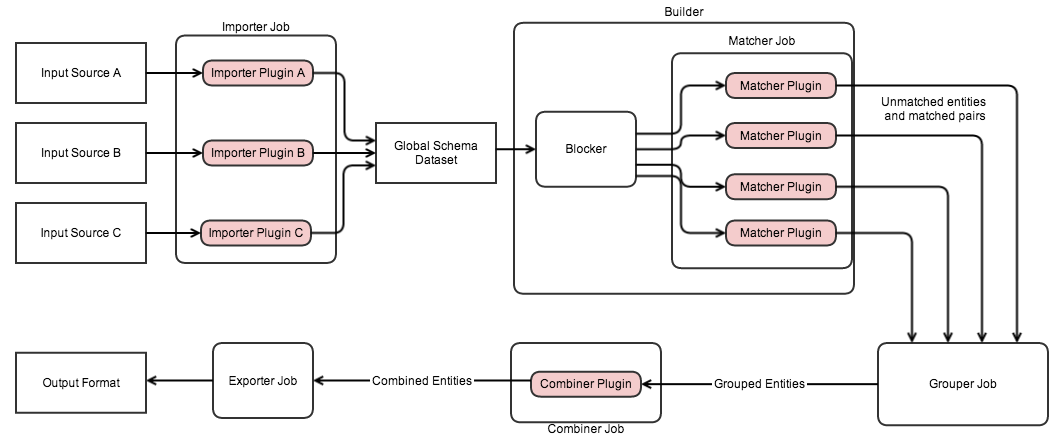
\includegraphics[scale=.5]{architecture}
%\end{figure}

First, a large dataset is converted into a set of common entities.
In this first stage, a dataset is fed into the normalizing stage, which is a MapReduce job in Java. Hadoop jobs already support many different file formats as inputs, and the framework will support them as well. Instead of extending the typical Runner/Mapper/Java classes for a job, the user will extend a class in the framework. In this subclass, the user will only need to define the relationship between the input data and the entity without writing redundant MapReduce boilerplate code.

In the second stage, all the entities generated in the first stage are pushed by the framework to the entity store in HBase. No deduplication or matching occurs at this stage, so the entity store may contain duplicates until the third stage. For particurlarly large datasets, the entity store may contain sparse data.

Finally, the entity store in HBase provides the input for the merging MapReduce job. Here, entities are matched together based on key attributes that are specified by the user. This may include fuzzy matching. The matched entities are referenced together in the reference table in HBase.

To utilize the framework, a user will include the framework Jar into their application. Then they will create a Java class to define the common entity. Java classes will be extended to provide infromation about each data source, entity relationships, and matching logic. Next, via a command on a Hadoop server, the framework will create the required infrastructure. Another command will integrate a specified source. A last command will merge, match, and provide the user with a unified output in a file.

\section{Recap}
The user defines:
\begin{itemize}
    \item The entity model and its attributes
    \item Relationships between input datasets and entities
    \item Key attributes to match and merge on between entities
    \item Thresholds of fuzzy and other heuristic matching devices
\end{itemize}

The Hadoop and HBase platform provide scaling capabilites, and my proposed framework provides the functionality for the in-between.

\section{Example}
The figure below is a concrete example of a use of the framework. The common "Programmer" entity is defined with a set of attributes. Large sets of heterogenous are fed into the framework, and data is fit to the entity model and pushed to HBase. Then, entities are matched (using email hashing here) and referenced as a single entity.\\
\includegraphics[scale=.5]{example}
\section{Implementation Schedule}
\begin{description}
    \item[Week 1] Additional architecture planning and finding test datasets
    \item[Week 2] Development of first stage framework and tools for normalizing data
    \item[Week 3] Testing first stage with datasets and using files as output (i.e. not HBase)
    \item[Week 4] Development of second stage framework and HBase table creation
    \item[Week 5] Testing first and second stage integration and verification of HBase contents
    \item[Week 6] Development of third stage framework MapReduce jobs -- matching and deduplication
    \item[Week 7] Implementation of advanced matching tools
    \item[Week 8] Application testing with good data
    \item[Week 9] Application testing with bad/malformed data -- improvement of error handling
    \item[Week 10] Demonstration and presentation
\end{description}
\section{Related Work}



\end{document}
